\documentclass[compress]{beamer}
\usepackage[utf8]{inputenc}
\usepackage[english]{babel}
\usepackage{hyperref}
\usepackage{ccicons}

\usepackage{tikz}
\usetikzlibrary{graphs, quotes, arrows.meta, matrix}

\usepackage{listings}
\lstset{language=Python}

\newcommand\scalemath[2]{\scalebox{#1}{\mbox{\ensuremath{\displaystyle #2}}}}

\usetheme{Ilmenau}
\usecolortheme{beaver}
\setbeamertemplate{navigation symbols}{}

\title{Graph theory}
\subtitle{Introduction and basic algorithms}
\author{Lorenzo Ferrari}
\institute{Campus Bornholm}
\date{\today}

\begin{document}

\begin{frame}[plain, fragile, t]
  \maketitle
  \begin{columns}
    \column{0.7\textwidth}
    \begin{flushleft}
      \small{\href{https://creativecommons.org/licenses/by-sa/4.0/}{This work is licensed under a Creative Commons Attribution-ShareAlike 4.0 International License}.}
    \end{flushleft}
    \column{0.2\textwidth}
    \begin{flushright}
      
\includegraphics[scale=0.7]{pics/by-sa.png}
    \end{flushright}
  \end{columns}
\end{frame}

\begin{frame}{Table of contents}
  \tableofcontents
\end{frame}

\AtBeginSection[]{
  \begin{frame}{Table of contents}
    \tableofcontents[currentsection]
  \end{frame}
}

\section{Introduction}

\subsection{Examples}

\begin{frame}{Examples}
  \begin{columns}
    \column{0.5\textwidth}
    \begin{center}
    \scalebox{0.7}{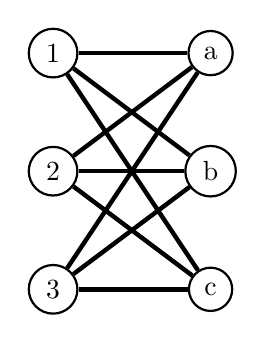
\begin{tikzpicture}
  \tikzset{vertex/.style = {draw, circle, thick}}
  \tikzset{arc/.style = {ultra thick}}
  % Nodes
  \node[vertex] (1) at (0, 3) {1};
  \node[vertex] (2) at (0, 1.5) {2};
  \node[vertex] (3) at (0, 0) {3};
  \node[vertex] (4) at (2, 3) {a};
  \node[vertex] (5) at (2, 1.5) {b};
  \node[vertex] (6) at (2, 0) {c};
  % Edges
  \draw[arc] (1) edge (4);
  \draw[arc] (1) edge (5);
  \draw[arc] (1) edge (6);
  \draw[arc] (2) edge (4);
  \draw[arc] (2) edge (5);
  \draw[arc] (2) edge (6);
  \draw[arc] (3) edge (4);
  \draw[arc] (3) edge (5);
  \draw[arc] (3) edge (6);
\end{tikzpicture}
}
    \end{center}
    \begin{center}
    \scalebox{0.7}{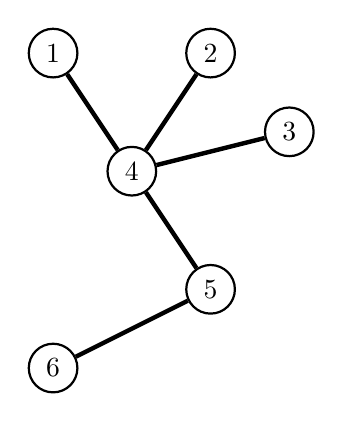
\begin{tikzpicture}
  \tikzset{vertex/.style = {draw, circle, thick}}
  \tikzset{arc/.style = {ultra thick}}
  % Nodes
  \node[vertex] (1) at (0, 4) {1};
  \node[vertex] (2) at (2, 4) {2};
  \node[vertex] (3) at (3, 3) {3};
  \node[vertex] (4) at (1, 2.5) {4};
  \node[vertex] (5) at (2, 1) {5};
  \node[vertex] (6) at (0, 0) {6};
  % Edges
  \draw[arc] (1) edge (4);
  \draw[arc] (2) edge (4);
  \draw[arc] (3) edge (4);
  \draw[arc] (4) edge (5);
  \draw[arc] (5) edge (6);
\end{tikzpicture}
}
    \end{center}
    \column{0.5\textwidth}
    \begin{center}
    \scalebox{0.7}{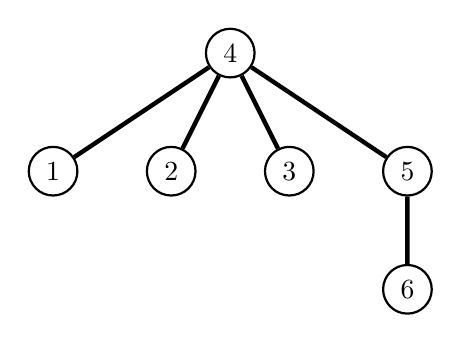
\begin{tikzpicture}
  \tikzset{vertex/.style = {draw, circle, thick}}
  \tikzset{arc/.style = {ultra thick}}
  % Actual tree
  \node[vertex] {4}
    child[arc] {node[vertex] {1}}
    child[arc] {node[vertex] {2}}
    child[arc] {node[vertex] {3}}
    child[arc] {node[vertex] {5}
      child[arc] {node[vertex] {6}}};
\end{tikzpicture}
}
    \end{center}
    \begin{center}
    \scalebox{0.7}{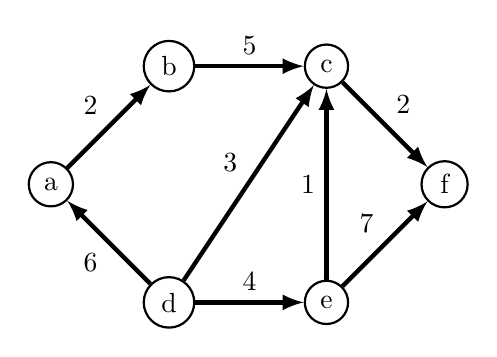
\begin{tikzpicture}
  \tikzset{vertex/.style = {draw, circle, thick}}
  \tikzset{arc/.style = {-latex, ultra thick}}
  % Nodes
  \node[vertex] (1) at (0, 1.5) {a};
  \node[vertex] (2) at (1.5, 3) {b};
  \node[vertex] (3) at (3.5, 3) {c};
  \node[vertex] (4) at (1.5, 0) {d};
  \node[vertex] (5) at (3.5, 0) {e};
  \node[vertex] (6) at (5, 1.5) {f};
  % Edges
  \draw[arc] (1) edge["2"] (2);
  \draw[arc] (2) edge["5"] (3);
  \draw[arc] (3) edge["2"] (6);
  \draw[arc] (4) edge["6"] (1);
  \draw[arc] (4) edge["3"] (3);
  \draw[arc] (4) edge["4"] (5);
  \draw[arc] (5) edge["1"] (3);
  \draw[arc] (5) edge["7"] (6);
\end{tikzpicture}
}
    \end{center}
  \end{columns}
\end{frame}

\begin{frame}[fragile]{Why graph theory?}
  \begin{alertblock}{}
    \begin{itemize}
    \item A huge number of problems can be converted in a graph problem
    \item Graph theory is fun \verb|\(^-^)/|
    \end{itemize}
  \end{alertblock}
  We will study problems in abstract form. Their application can be found in the most diverse areas.
\end{frame}

\begin{frame}{Typical graphs problems}
  \begin{itemize}
  \item Given the description of a city, find the shortest path between locations $A$ and $B$ or determine that it is impossible to reach $B$ from $A$.
  \item On an electronic board, choose a set of connections whose sum in length is minimal and which allows to pass through all points of interest.
  \item Given dependency relationships, find a suitable order to install some packages (or attend some classes) or determine that it is impossible.
  \end{itemize}
\end{frame}

\subsection{Definitions}
\begin{frame}{Definition: Graph}
  \begin{block}{\textbf{Graph} $G = (V, E)$}
    A graph is defined as a pair of sets:
    \begin{itemize}
    \item $V$ is a set of {\color{red}vertexes}/{\color{red}nodes}
    \item $E$ is a set of {\color{red}edges}
  \end{itemize}
\end{block}
\end{frame}

\begin{frame}{Definition: Vertexes and Edges}
  \begin{block}{\textbf{Vertex}}
      \begin{itemize}
      \item Vertexes are also called \emph{nodes}
      \item Vertexes are denoted with labels
    \end{itemize}
  \end{block}
  \begin{block}{\textbf{Edge}}
      \begin{itemize}
      \item Each edge is defined by a pair of vertexes
      \item An edge \emph{connects} the vertexes that define it
      \item In some cases, the vertexes can be the same
  \end{itemize}
\end{block}
\end{frame}

\begin{frame}{}
  \begin{example}
    \begin{itemize}
    \item $G = (V, E)$
    \item $V = \{1, 2, 3, 4\}$
    \item $E = \{(1,2), (1,3), (1,4), (2,4), (3,4)\}$
    \end{itemize}
  \end{example}
  \begin{center}
  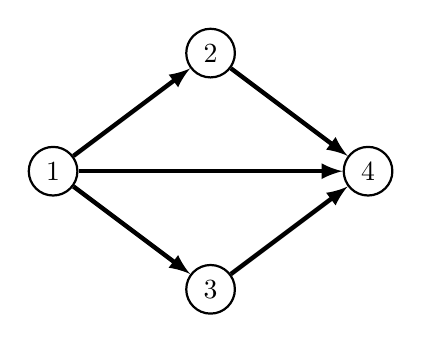
\begin{tikzpicture}
  \tikzset{vertex/.style = {draw, circle, thick}}
  \tikzset{arc/.style = {-latex, ultra thick}}
  % Nodes
  \node[vertex] (1) at (0, 2) {1};
  \node[vertex] (2) at (2, 3.5) {2};
  \node[vertex] (3) at (2, 0.5) {3};
  \node[vertex] (4) at (4, 2) {4};
  % Edges
  \draw[arc] (1) edge (2);
  \draw[arc] (1) edge (3);
  \draw[arc] (1) edge (4);
  \draw[arc] (2) edge (4);
  \draw[arc] (3) edge (4);
\end{tikzpicture}

  \end{center}
\end{frame}

\begin{frame}{Definition: Paths and Cycles}
  \begin{block}{\textbf{Path}}
    A path of length $n$ in a graph $G = (V, E)$ is a sequence $v_0, \dots, v_n \in V$ such that $(v_{i-1}, v_i) \in E \ \forall \ 1 \leq i \leq r$. \\

    A path is \emph{simple} if all $v_i$ differ.
  \end{block}
  \begin{block}{\textbf{Cycle}}
    A cycle is a path in which the first and the last node are the same.
  \end{block}
\end{frame}

\begin{frame}{Definition: Subgraph}
  \begin{block}{\textbf{Subgraph}}
    A graph $G' = (V', E')$ is subgraph of $G = (V, E)$ if $V' \subseteq V$ and $E' \subseteq E$.
  \end{block}
  \begin{columns}
  \column{0.5\textwidth}
  \begin{center}
  \scalebox{0.7}{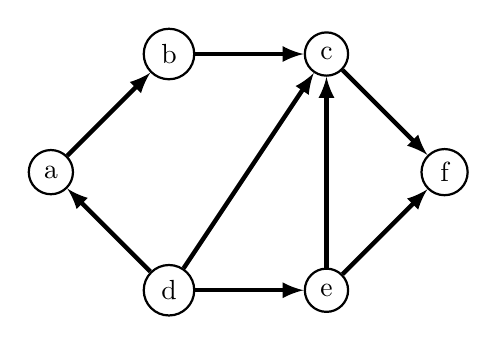
\begin{tikzpicture}
  \tikzset{vertex/.style = {draw, circle, thick}}
  \tikzset{arc/.style = {-latex, ultra thick}}
  % Nodes
  \node[vertex] (1) at (0, 1.5) {a};
  \node[vertex] (2) at (1.5, 3) {b};
  \node[vertex] (3) at (3.5, 3) {c};
  \node[vertex] (4) at (1.5, 0) {d};
  \node[vertex] (5) at (3.5, 0) {e};
  \node[vertex] (6) at (5, 1.5) {f};
  % Edges
  \draw[arc] (1) edge (2);
  \draw[arc] (2) edge (3);
  \draw[arc] (3) edge (6);
  \draw[arc] (4) edge (1);
  \draw[arc] (4) edge (3);
  \draw[arc] (4) edge (5);
  \draw[arc] (5) edge (3);
  \draw[arc] (5) edge (6);
\end{tikzpicture}
}
  \end{center}
  \column{0.5\textwidth}
  \begin{center}
  \scalebox{0.7}{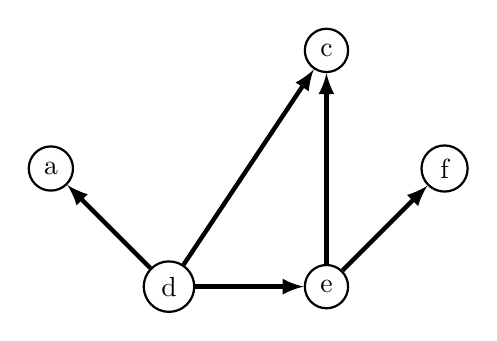
\begin{tikzpicture}
  \tikzset{vertex/.style = {draw, circle, thick}}
  \tikzset{arc/.style = {-latex, ultra thick}}
  % Nodes
  \node[vertex] (1) at (0, 1.5) {a};
  % \node[vertex] (2) at (1.5, 3) {b};
  \node[vertex] (3) at (3.5, 3) {c};
  \node[vertex] (4) at (1.5, 0) {d};
  \node[vertex] (5) at (3.5, 0) {e};
  \node[vertex] (6) at (5, 1.5) {f};
  % Edges
  % \draw[arc] (1) edge (2);
  % \draw[arc] (2) edge (3);
  % \draw[arc] (3) edge (6);
  \draw[arc] (4) edge (1);
  \draw[arc] (4) edge (3);
  \draw[arc] (4) edge (5);
  \draw[arc] (5) edge (3);
  \draw[arc] (5) edge (6);
\end{tikzpicture}
}
  \end{center}
  \end{columns}
\end{frame}

\subsection{Kinds of graph}
\begin{frame}[fragile]{Directed and Undirected graphs}
  \begin{columns}
  \column{0.5\textwidth}
  \begin{block}{\textbf{Directed graph} $G = (V, E)$}
    \begin{itemize}
      \item $E$ is a set of \emph{ordered} pairs $(u, v)$ of nodes
    \end{itemize}
  \end{block}
  \begin{verbatim}
V = { a,b,c,d,e,f }
E = { (a,b),(a,d),(b,c),
      (d,a),(d,c),(d,e),
      (e,c) }
  \end{verbatim}
  \begin{center}
  \scalebox{0.65}{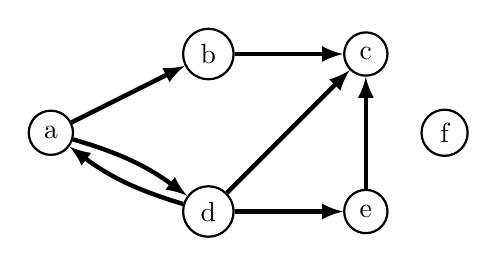
\begin{tikzpicture}
  \tikzset{vertex/.style = {draw, circle, thick}}
  \tikzset{arc/.style = {-latex, ultra thick}}
  % Nodes
  \node[vertex] (1) at (0, 1) {a};
  \node[vertex] (2) at (2, 2) {b};
  \node[vertex] (3) at (4, 2) {c};
  \node[vertex] (4) at (2, 0) {d};
  \node[vertex] (5) at (4, 0) {e};
  \node[vertex] (6) at (5, 1) {f};
  % Edges
  \draw[arc] (1) edge (2);
  \draw[arc] (2) edge (3);
  \draw[arc] (4) edge (3);
  \draw[arc] (4) edge (5);
  \draw[arc] (5) edge (3);
  \draw[arc, bend left = 10] (1) edge (4);
  \draw[arc, bend left = 10] (4) edge (1);
\end{tikzpicture}
}
  \end{center}
  \column{0.5\textwidth}
  \begin{block}{\textbf{Undirected graph} $G = (V, E)$}
    \begin{itemize}
      \item $E$ is a set of \emph{unordered} pairs $[u, v]$ of nodes
    \end{itemize}
  \end{block}
  \begin{verbatim}
V = { a,b,c,d,e,f }
E = { [a,b],[a,d],[b,c],
      [c,d],[c,e],[e,d] }

  \end{verbatim}
  \begin{center}
  \scalebox{0.65}{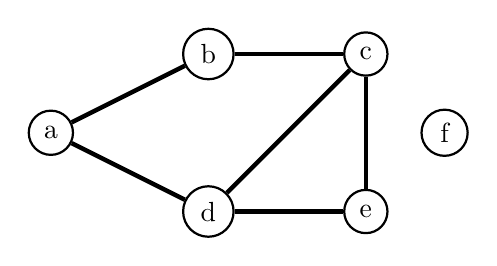
\begin{tikzpicture}
  \tikzset{vertex/.style = {draw, circle, thick}}
  \tikzset{arc/.style = {ultra thick}}
  % Nodes
  \node[vertex] (1) at (0, 1) {a};
  \node[vertex] (2) at (2, 2) {b};
  \node[vertex] (3) at (4, 2) {c};
  \node[vertex] (4) at (2, 0) {d};
  \node[vertex] (5) at (4, 0) {e};
  \node[vertex] (6) at (5, 1) {f};
  % Edges
  \draw[arc] (1) edge (2);
  \draw[arc] (2) edge (3);
  \draw[arc] (4) edge (3);
  \draw[arc] (4) edge (5);
  \draw[arc] (5) edge (3);
  \draw[arc] (1) edge (4);
\end{tikzpicture}
}
  \end{center}
\end{columns}
\end{frame}

\begin{frame}{Cyclic and Acyclic graphs}
  \begin{columns}
    \column{0.5\textwidth}
    \begin{block}{\textbf{Cyclic graph}}
      \begin{itemize}
        \item Contains cycles
      \end{itemize}
    \end{block}
    \begin{center}
    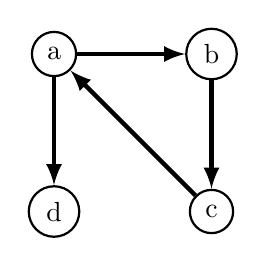
\begin{tikzpicture}
  \tikzset{vertex/.style = {draw, circle, thick}}
  \tikzset{arc/.style = {-latex, ultra thick}}
  % Nodes
  \node[vertex] (1) at (0, 2) {a};
  \node[vertex] (2) at (2, 2) {b};
  \node[vertex] (3) at (2, 0) {c};
  \node[vertex] (4) at (0, 0) {d};
  % Edges
  \draw[arc] (1) edge (2);
  \draw[arc] (1) edge (4);
  \draw[arc] (2) edge (3);
  \draw[arc] (3) edge (1);
\end{tikzpicture}

  \end{center}
    \column{0.5\textwidth}
    \begin{block}{\textbf{Acyclic graph}}
      \begin{itemize}
        \item Contains no cycles
      \end{itemize}
    \end{block}
    \begin{center}
    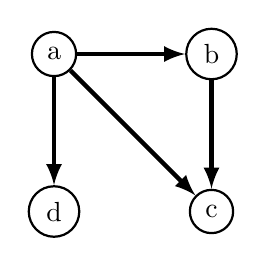
\begin{tikzpicture}
  \tikzset{vertex/.style = {draw, circle, thick}}
  \tikzset{arc/.style = {-latex, ultra thick}}
  % Nodes
  \node[vertex] (1) at (0, 2) {a};
  \node[vertex] (2) at (2, 2) {b};
  \node[vertex] (3) at (2, 0) {c};
  \node[vertex] (4) at (0, 0) {d};
  % Edges
  \draw[arc] (1) edge (2);
  \draw[arc] (1) edge (4);
  \draw[arc] (1) edge (3);
  \draw[arc] (2) edge (3);
\end{tikzpicture}

    \end{center}
  \end{columns}
\end{frame}

\begin{frame}{Cyclic and Acyclic graphs}
  \begin{columns}
    \column{0.5\textwidth}
    \begin{block}{\textbf{Cyclic graph}}
      \begin{itemize}
        \item Contains cycles
      \end{itemize}
    \end{block}
    \begin{center}
    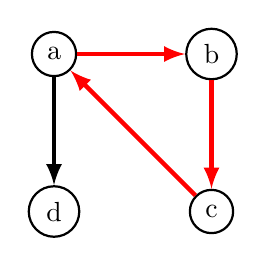
\begin{tikzpicture}
  \tikzset{vertex/.style = {draw, circle, thick}}
  \tikzset{arc/.style = {-latex, ultra thick}}
  % Nodes
  \node[vertex] (1) at (0, 2) {a};
  \node[vertex] (2) at (2, 2) {b};
  \node[vertex] (3) at (2, 0) {c};
  \node[vertex] (4) at (0, 0) {d};
  % Edges
  \draw[arc] (1) edge[red] (2);
  \draw[arc] (1) edge (4);
  \draw[arc] (2) edge[red] (3);
  \draw[arc] (3) edge[red] (1);
\end{tikzpicture}

  \end{center}
    \column{0.5\textwidth}
    \begin{block}{\textbf{Acyclic graph}}
      \begin{itemize}
        \item Contains no cycles
      \end{itemize}
    \end{block}
    \begin{center}
    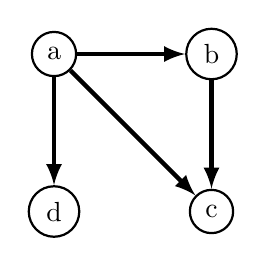
\begin{tikzpicture}
  \tikzset{vertex/.style = {draw, circle, thick}}
  \tikzset{arc/.style = {-latex, ultra thick}}
  % Nodes
  \node[vertex] (1) at (0, 2) {a};
  \node[vertex] (2) at (2, 2) {b};
  \node[vertex] (3) at (2, 0) {c};
  \node[vertex] (4) at (0, 0) {d};
  % Edges
  \draw[arc] (1) edge (2);
  \draw[arc] (1) edge (4);
  \draw[arc] (1) edge (3);
  \draw[arc] (2) edge (3);
\end{tikzpicture}

    \end{center}
  \end{columns}
\end{frame}

\begin{frame}{Weighted graphs}
  \begin{block}{\textbf{Weighted graph}}
    \begin{itemize}
      \item Each edge is assigned a \emph{wheight}
      \item Weigth typically shows cost of traversing
    \end{itemize}
  \end{block}
  \begin{center}
  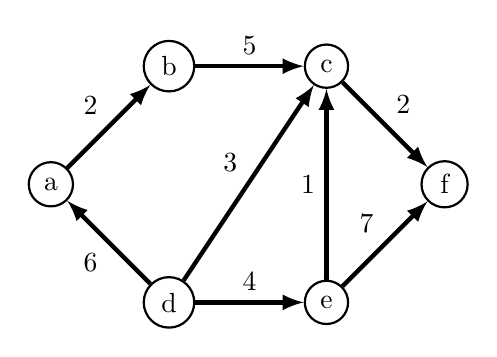
\begin{tikzpicture}
  \tikzset{vertex/.style = {draw, circle, thick}}
  \tikzset{arc/.style = {-latex, ultra thick}}
  % Nodes
  \node[vertex] (1) at (0, 1.5) {a};
  \node[vertex] (2) at (1.5, 3) {b};
  \node[vertex] (3) at (3.5, 3) {c};
  \node[vertex] (4) at (1.5, 0) {d};
  \node[vertex] (5) at (3.5, 0) {e};
  \node[vertex] (6) at (5, 1.5) {f};
  % Edges
  \draw[arc] (1) edge["2"] (2);
  \draw[arc] (2) edge["5"] (3);
  \draw[arc] (3) edge["2"] (6);
  \draw[arc] (4) edge["6"] (1);
  \draw[arc] (4) edge["3"] (3);
  \draw[arc] (4) edge["4"] (5);
  \draw[arc] (5) edge["1"] (3);
  \draw[arc] (5) edge["7"] (6);
\end{tikzpicture}

  \end{center}
\end{frame}

\begin{frame}{Trees}
  \begin{columns}
    \column{0.5\textwidth}
    \begin{block}{\textbf{Tree}}
      \begin{itemize}
      \item \emph{Connected} graph with $m = n - 1$
      \end{itemize}
    \end{block}
    \begin{center}
    \scalebox{0.7}{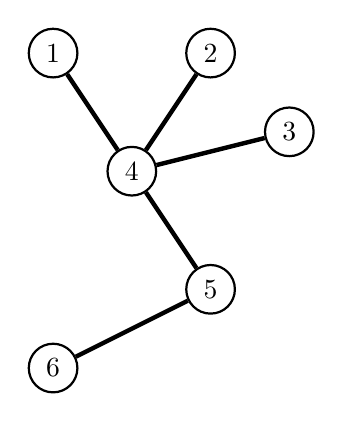
\begin{tikzpicture}
  \tikzset{vertex/.style = {draw, circle, thick}}
  \tikzset{arc/.style = {ultra thick}}
  % Nodes
  \node[vertex] (1) at (0, 4) {1};
  \node[vertex] (2) at (2, 4) {2};
  \node[vertex] (3) at (3, 3) {3};
  \node[vertex] (4) at (1, 2.5) {4};
  \node[vertex] (5) at (2, 1) {5};
  \node[vertex] (6) at (0, 0) {6};
  % Edges
  \draw[arc] (1) edge (4);
  \draw[arc] (2) edge (4);
  \draw[arc] (3) edge (4);
  \draw[arc] (4) edge (5);
  \draw[arc] (5) edge (6);
\end{tikzpicture}
}
    \end{center}
    \column{0.5\textwidth}
    \begin{block}{\textbf{Rooted tree}}
      \begin{itemize}
      \item \emph{Connected} graph with $m = n - 1$ in which some special node is designed as root
      \end{itemize}
    \end{block}
    \begin{center}
    \scalebox{0.8}{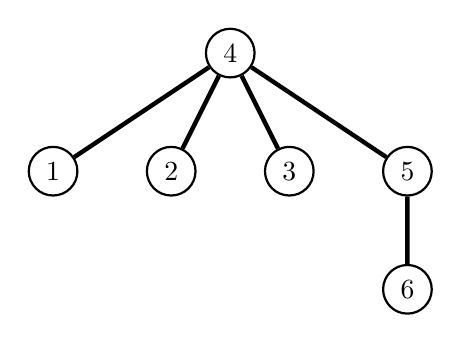
\begin{tikzpicture}
  \tikzset{vertex/.style = {draw, circle, thick}}
  \tikzset{arc/.style = {ultra thick}}
  % Actual tree
  \node[vertex] {4}
    child[arc] {node[vertex] {1}}
    child[arc] {node[vertex] {2}}
    child[arc] {node[vertex] {3}}
    child[arc] {node[vertex] {5}
      child[arc] {node[vertex] {6}}};
\end{tikzpicture}
}
    \end{center}
  \end{columns}
\end{frame}

\subsection{Graph representation}

\begin{frame}{Representations}
  \begin{block}{}
    Two possible "classic" implementations
  \end{block}
  \begin{itemize}
    \item Adjacency matrix
    \item Adjacency list
  \end{itemize}
\end{frame}

\begin{frame}{Adjacency matrix}
  \begin{columns}
    \column{0.5\textwidth}
    \[
    m_{uv} = \begin{cases}
      1, & \text{if $(u,v) \in E$} \\
      0, & \text{if $(u,v) \notin E$}
    \end{cases}
    \]
    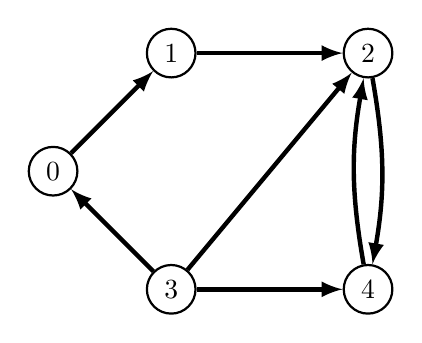
\begin{tikzpicture}
  \tikzset{vertex/.style = {draw, circle, thick}}
  \tikzset{arc/.style = {-latex, ultra thick}}
  % Nodes
  \node[vertex] (1) at (0, 1.5) {0};
  \node[vertex] (2) at (1.5, 3) {1};
  \node[vertex] (3) at (4, 3) {2};
  \node[vertex] (4) at (1.5, 0) {3};
  \node[vertex] (5) at (4, 0) {4};
  % \node[vertex] (6) at (5, 1.5) {5};
  % Edges
  \draw[arc] (1) edge (2);
  \draw[arc] (2) edge (3);
  % \draw[arc] (3) edge (6);
  \draw[arc] (4) edge (1);
  \draw[arc] (4) edge (3);
  \draw[arc] (4) edge (5);
  \draw[arc] (5) edge[bend left = 10] (3);
  \draw[arc] (3) edge[bend left = 10] (5);
  % \draw[arc] (5) edge (6);
\end{tikzpicture}

    \column{0.5\textwidth}
    \[
    \begin{matrix}
       & \textbf{0} & \textbf{1} & \textbf{2} & \textbf{3} & \textbf{4} \\
      \textbf{0} & 0 & 1 & 0 & 0 & 0 \\
      \textbf{1} & 0 & 0 & 1 & 0 & 0 \\
      \textbf{2} & 0 & 0 & 0 & 0 & 1 \\
      \textbf{3} & 1 & 0 & 1 & 0 & 1 \\
      \textbf{4} & 0 & 0 & 1 & 0 & 0
    \end{matrix}
    \]
  \end{columns}
\end{frame}

\begin{frame}{Adjacency list}
  \begin{columns}
  \column{0.5\textwidth}
  \[G.adj(u) = \{v \ | \ (u,v) \in E\}\]
  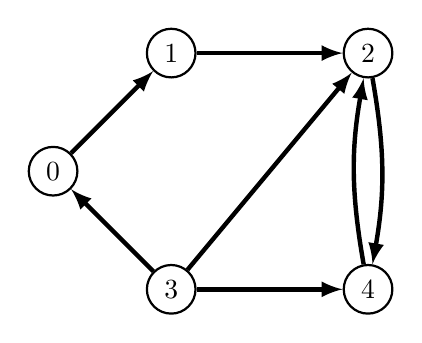
\begin{tikzpicture}
  \tikzset{vertex/.style = {draw, circle, thick}}
  \tikzset{arc/.style = {-latex, ultra thick}}
  % Nodes
  \node[vertex] (1) at (0, 1.5) {0};
  \node[vertex] (2) at (1.5, 3) {1};
  \node[vertex] (3) at (4, 3) {2};
  \node[vertex] (4) at (1.5, 0) {3};
  \node[vertex] (5) at (4, 0) {4};
  % \node[vertex] (6) at (5, 1.5) {5};
  % Edges
  \draw[arc] (1) edge (2);
  \draw[arc] (2) edge (3);
  % \draw[arc] (3) edge (6);
  \draw[arc] (4) edge (1);
  \draw[arc] (4) edge (3);
  \draw[arc] (4) edge (5);
  \draw[arc] (5) edge[bend left = 10] (3);
  \draw[arc] (3) edge[bend left = 10] (5);
  % \draw[arc] (5) edge (6);
\end{tikzpicture}

  \column{0.5\textwidth}
  $\scalemath{1.8}{\fbox{0} \rightarrow \fbox{1}}$ \\
  $\scalemath{1.8}{\fbox{1} \rightarrow \fbox{2}}$ \\
  $\scalemath{1.8}{\fbox{2} \rightarrow \fbox{4}}$ \\
  $\scalemath{1.8}{\fbox{3} \rightarrow \fbox{0}\fbox{2}\fbox{4}}$ \\
  $\scalemath{1.8}{\fbox{4} \rightarrow \fbox{2}}$
  \end{columns}
\end{frame}

\section{Graph traversals}

\subsection{BFS}
\begin{frame}{Breadth-first search}
  \begin{block}{\textbf{Problem definition}}
    Given a graph $G = (V, E)$ and a vertex $r \in V$ (root), visit exactly once all the vertexes of the graph that can be reached from $r$.
  \end{block}
  \begin{block}{\textbf{Breadth-first search (BFS)}}
    Traverse the graph by visiting the nodes by levels: first nodes at distance 1 from the source, then distance 2, etc.
    \begin{itemize}
    \item Application: shortest distances
    \end{itemize}
  \end{block}
\end{frame}

\begin{frame}[fragile]{Breadth-first search}
\begin{lstlisting}
def bfs(G, r):
  Q = deque()
  Q.append(r)
  visited = {r}
  while len(Q) > 0:
    u = Q.popleft()
    for v in G.adj(u):
      if not v in visited:
        visited.add(v)
        Q.append(v)
\end{lstlisting}
\end{frame}

\subsection{DFS}
\begin{frame}{Depth-first search}
  \begin{block}{\textbf{Problem definition}}
    Given a graph $G = (V, E)$ and a vertex $r \in V$ (root), visit exactly once all the vertexes of the graph that can be reached from $r$.
  \end{block}
  \begin{block}{\textbf{Depth-first search (DFS)}}
    Traverse the graph by visiting all the nodes that can be reached by a node, and all the nodes that can be reached by those nodes, etc.
    \begin{itemize}
    \item Application: topological sort
    \item Application: cycle detection
    \item Application: connected components
    \item Application: strongly connected components
    \end{itemize}
  \end{block}
\end{frame}

\begin{frame}[fragile]{Depth-first search: iterative}
\begin{lstlisting}
def dfs(G, r):
  stack = [r]
  visited = {r}
  while len(st) > 0:
    u = stack.pop()
    for v in G.adj(u):
      if not v in visited:
        visited.add(v)
        stack.append(v)
\end{lstlisting}
\end{frame}

\begin{frame}[fragile]{Depth-first search: recursive}
\begin{lstlisting}
def dfs(G, u, visited):
  visited.add(r)
  for v in G.adj(u):
    if not v in visited
      dfs(G, v, visited)
\end{lstlisting}
\end{frame}

\section{Problems}

\subsection{MST}
\begin{frame}{Minimum Spanning Tree (MST)}
  \begin{block}{\textbf{Problem definition}}
    Given a connected weighted graph $G = (V, E)$, find $S \subseteq E$ such that $(V, S)$ is still connected and $S$ has the minimum total edge weight.
  \end{block}
  \begin{center}
  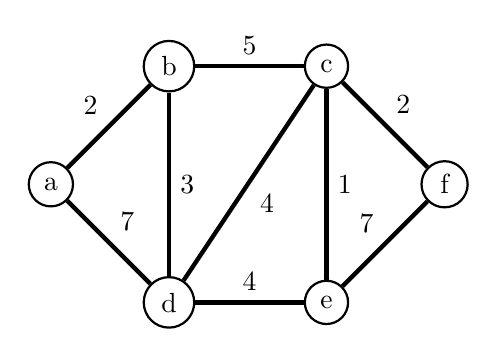
\begin{tikzpicture}
  \tikzset{vertex/.style = {draw, circle, thick}}
  \tikzset{arc/.style = {ultra thick}}
  % Nodes
  \node[vertex] (1) at (0, 1.5) {a};
  \node[vertex] (2) at (1.5, 3) {b};
  \node[vertex] (3) at (3.5, 3) {c};
  \node[vertex] (4) at (1.5, 0) {d};
  \node[vertex] (5) at (3.5, 0) {e};
  \node[vertex] (6) at (5, 1.5) {f};
  % Edges
  \draw[arc] (1) edge["2"] (2);
  \draw[arc] (1) edge["7"] (4);
  \draw[arc] (2) edge["5"] (3);
  \draw[arc] (2) edge["3"] (4);
  \draw[arc] (3) edge["2"] (6);
  \draw[arc] (3) edge["4"] (4);
  \draw[arc] (3) edge["1"] (5);
  \draw[arc] (4) edge["4"] (5);
  \draw[arc] (5) edge["7"] (6);
\end{tikzpicture}

  \end{center}
\end{frame}

\begin{frame}{Minimum Spanning Tree (MST)}
  \begin{block}{\textbf{Problem definition}}
    Given a connected weighted graph $G = (V, E)$, find $S \subseteq E$ such that $(V, S)$ is still connected and $S$ has the minimum total edge weight.
  \end{block}
  \begin{center}
  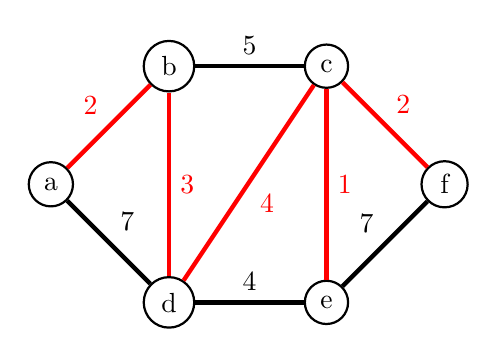
\begin{tikzpicture}
  \tikzset{vertex/.style = {draw, circle, thick}}
  \tikzset{arc/.style = {ultra thick}}
  % Nodes
  \node[vertex] (1) at (0, 1.5) {a};
  \node[vertex] (2) at (1.5, 3) {b};
  \node[vertex] (3) at (3.5, 3) {c};
  \node[vertex] (4) at (1.5, 0) {d};
  \node[vertex] (5) at (3.5, 0) {e};
  \node[vertex] (6) at (5, 1.5) {f};
  % Edges
  \draw[arc] (1) edge["2", red] (2);
  \draw[arc] (1) edge["7"] (4);
  \draw[arc] (2) edge["5"] (3);
  \draw[arc] (2) edge["3", red] (4);
  \draw[arc] (3) edge["2", red] (6);
  \draw[arc] (3) edge["4", red] (4);
  \draw[arc] (3) edge["1", red] (5);
  \draw[arc] (4) edge["4"] (5);
  \draw[arc] (5) edge["7"] (6);
\end{tikzpicture}

  \end{center}
\end{frame}

\begin{frame}[fragile]{Kruskal algorithm for MST}
\begin{lstlisting}
def mst(E):
  E.sort()  # sort for increasing weight
  ans = []
  for edge in E:
    if not Cycle(ans, edge):
      ans.append(edge)

  return ans
\end{lstlisting}
\end{frame}

\subsection{Connected components}
\begin{frame}{Connected Components}
  \begin{block}{\textbf{Problem definition}}
    Given an undirected graph $G = (V, E)$, find the number of connected components.
  \end{block}
  \begin{center}
  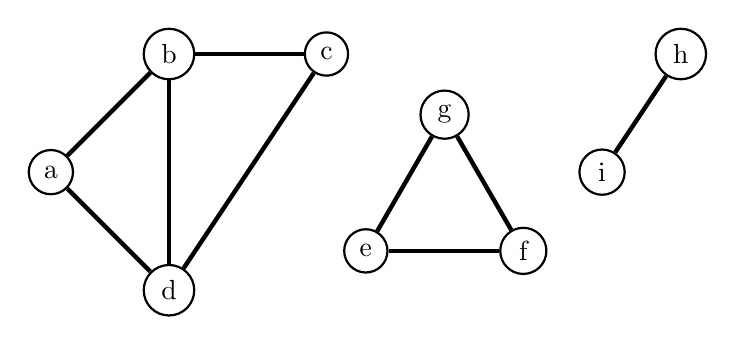
\begin{tikzpicture}
  \tikzset{vertex/.style = {draw, circle, thick}}
  \tikzset{arc/.style = {ultra thick}}
  % Component 1
  \node[vertex] (1) at (0, 1.5) {a};
  \node[vertex] (2) at (1.5, 3) {b};
  \node[vertex] (3) at (3.5, 3) {c};
  \node[vertex] (4) at (1.5, 0) {d};
  \draw[arc] (1) edge (2);
  \draw[arc] (1) edge (4);
  \draw[arc] (2) edge (3);
  \draw[arc] (2) edge (4);
  \draw[arc] (3) edge (4);
  % work in progress
  % \draw[blue, dashed, rounded corners = 8pt] (1) -- (2) -- (3) -- (4) -- (1);
  % Component 2
  \node[vertex] (5) at (4, 0.5) {e};
  \node[vertex] (6) at (6, 0.5) {f};
  \node[vertex] (7) at (5, 2.23) {g};
  \draw[arc] (5) edge (6);
  \draw[arc] (5) edge (7);
  \draw[arc] (6) edge (7);
  % Component 3
  \node[vertex] (8) at (8, 3) {h};
  \node[vertex] (9) at (7, 1.5) {i};
  \draw[arc] (8) edge (9);
\end{tikzpicture}

  \end{center}
\end{frame}

\begin{frame}[fragile]{Connected Components}
\begin{lstlisting}
def connectedComponents(G):
  visited = {}
  count = 0
  for u in G.V:
    if not u in visited:
      count += 1
      dfs(G, u, visited)

  return count
\end{lstlisting}
\end{frame}

\subsection{Single source shortest path}
\begin{frame}{Single source shortest path}
  \begin{block}{\textbf{Problem definition}}
    Given a weigthed graph $G = (V, E)$ and a source node $s$, find the distance of every node from $s$. If there is not a path from $s$ to a node $v$, \texttt{dist[v]} should be $+\infty$.
  \end{block}
  \begin{center}
  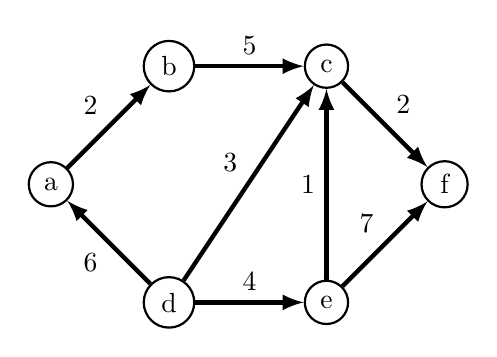
\begin{tikzpicture}
  \tikzset{vertex/.style = {draw, circle, thick}}
  \tikzset{arc/.style = {-latex, ultra thick}}
  % Nodes
  \node[vertex] (1) at (0, 1.5) {a};
  \node[vertex] (2) at (1.5, 3) {b};
  \node[vertex] (3) at (3.5, 3) {c};
  \node[vertex] (4) at (1.5, 0) {d};
  \node[vertex] (5) at (3.5, 0) {e};
  \node[vertex] (6) at (5, 1.5) {f};
  % Edges
  \draw[arc] (1) edge["2"] (2);
  \draw[arc] (2) edge["5"] (3);
  \draw[arc] (3) edge["2"] (6);
  \draw[arc] (4) edge["6"] (1);
  \draw[arc] (4) edge["3"] (3);
  \draw[arc] (4) edge["4"] (5);
  \draw[arc] (5) edge["1"] (3);
  \draw[arc] (5) edge["7"] (6);
\end{tikzpicture}

  \end{center}
\end{frame}

\begin{frame}[fragile]{Single source shortest path}
\begin{lstlisting}
def shortestPath(G, s):
  Q = deque()
  dist = [math.inf] * G.n
  dist[s] = 0
  Q.append(s)
  while len(Q) > 0:
    u = Q.popleft()
    for (v,w) in G.adj(u):
      if dist[v] > dist[u] + w
        dist[v] = dist[u] + w
        Q.append(v)

  return dist
\end{lstlisting}
\end{frame}

\subsection{Conclusion}

\begin{frame}{More problems}
  \begin{itemize}
  \item Given an undirected graph, find the minimum number of edges to add if you want to make it connected.
  \item Given a weighted graph and three nodes $a, b, c$, find a minimal length path which goes from $a$ to $c$ passing through $b$.
  \item Given a directed graph, find a permutation of $V$ such that $\forall \ (u,v) \in E$ $u$ comes before $v$, or tell it is impossible.
  \item Given a set of words $S$, find a minimal length string which contains each element of $S$ as a substring.
  \item Given some dominoes, tell whether you can put them in a line such that the domino condition is satisfied.
  \end{itemize}
\end{frame}

\begin{frame}{Any questions?}
  \tableofcontents
\end{frame}

\end{document}

% https://www.radford.edu/nokie/classes/360/graphs-terms.html
% http://disi.unitn.it/~montreso/python/B04-grafi.pdf
% https://www.olimpiadi-informatica.it/files/guida_selezioni%20territoriali.pdf
